\documentclass[10pt, unicode]{beamer}

% set font
\usepackage{fontspec}
\setsansfont{Fira Sans}
\newfontfamily\cyrillicfont{Fira Sans}

% set lang
\usepackage{polyglossia}
\setdefaultlanguage[spelling=modern]{russian}
\setotherlanguage{english}

% set theme
\usetheme{metropolis}

% packages
\usepackage{caption}

% set info
\title{Рекомендательная система для VLru Еда}
\author{
    Студент: \\ Сластен Тихон Дмитриевич \\ \\
    Руководитель: \\ Старший преподаватель ИМКМ Кленин Александр Сергеевич}
\institute{Б8403а Прикладная математика и информатика}
\date{}

\begin{document}

% Заголовок
\maketitle

\begin{frame}
  \frametitle{Проект "VLru Еда"}
  \begin{itemize}
    \item Начал свою работу в апреле 2018 года
    \item Более 100 компаний
    \item Около 8000 блюд
    \item Также, проект существует в Хабаровске под названием "DVHAB Еда"
  \end{itemize}
\end{frame}

\begin{frame}
  \frametitle{Цель работы}
  Разработать и внедрить на сайт VLru Еда рекомендательную систему
\end{frame}

\begin{frame}
  \frametitle{Структура данных}
  \begin{figure}[H]
    \centering
    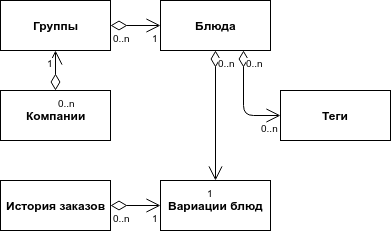
\includegraphics[scale=0.6]{images/database.png}
    \caption{Структура базы данных}
  \end{figure}
\end{frame}

\begin{frame}
  \frametitle{Коллаборативная фильтрация}
  \begin{itemize}
    \item $I_u$ - множество товаров, которые оценил пользователь $u$
    \item $U_i$ - множество пользователей, которые оценили товар $i$
    \item $SIM(i,j)$ - функция схожести товаров $i$ и $j$
    \item $r_{ij}$ - оценка пользователя $u$ товару $i$
  \end{itemize}
\end{frame}

\begin{frame}
  \frametitle{Item-based коллаборативная фильтрация}
  \begin{columns}[T]
    \begin{column}{.6\textwidth}
     		\begin{enumerate}
          \item Коэффициент Жаккара
          \begin{align*}
            JS(i,j) = \frac{|U_i \cap U_j|}{|U_i \cup U_j|}
          \end{align*}
          \item Косинусное сходство
          \begin{align*}
            CS(i,j) = \frac{\sum_{u \in U_{ij}} r_{ui}r_{uj}}{\sqrt{\sum_{u \in U_{ij}} r_{ui}^2}\sqrt{\sum_{u \in U_{ij}} r_{uj}^2}}
          \end{align*}
          \item Коэффициент корреляции Пирсона
          \begin{align*}
            PS(i,j) = \frac
              {\sum_{u \in U_{ij}} (r_{ui} - \hat{r}_i)(r_{uj} - \hat{r}_j)}
              {\sqrt{\sum_{u \in U_{ij}} (r_{ui} - \hat{r}_i)^2}\sqrt{\sum_{u \in U_{ij}} (r_{uj} - \hat{r}_j)^2}}
          \end{align*}
        \end{enumerate}
    	\end{column}
    	\begin{column}{.4\textwidth}
    		\begin{figure}
    			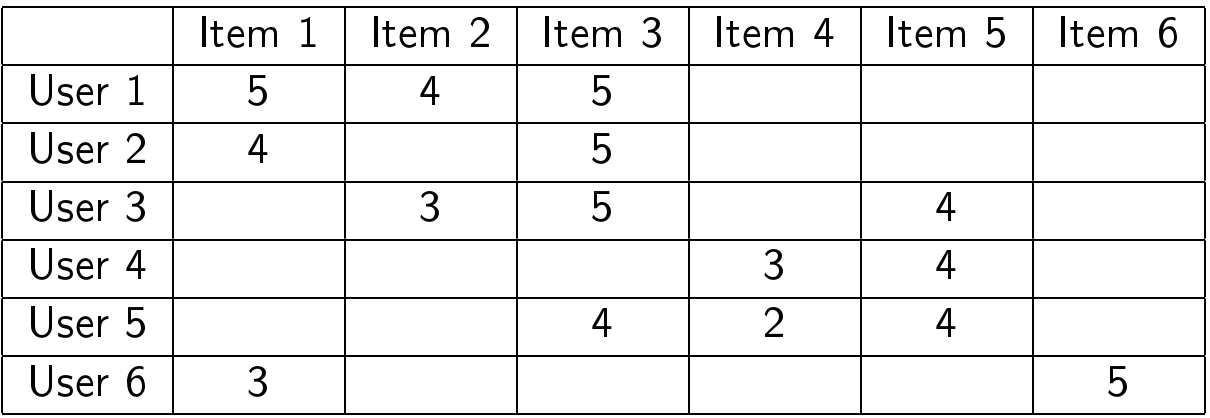
\includegraphics[width=\textwidth]{images/user_item.png}
    			\caption{Таблица оценок пользователей}
    		\end{figure}
      \end{column}
  \end{columns}
\end{frame}

\begin{frame}
  \frametitle{Вычисление предсказаний}
  \begin{enumerate}
    \item Коэффициент Жаккара
    \begin{align*}
      \hat{r}_{uj} = \frac{\sum_{i \in I_u} SIM(i,j)}{|I_u|}
    \end{align*}
    \item Косинусное сходство
    \begin{align*}
      \hat{r}_{uj} = \frac{\sum_{i \in I_u} SIM(i,j) r_{ui} }{\sum_{i \in I_u} SIM(i,j)}
    \end{align*}
    \item Коэффициент корреляции Пирсона
    \begin{align*}
      \hat{r}_{uj} = \bar{r}_j + \frac{\sum_{i \in I_u} SIM(i,j) (r_{ui} - \bar{r}_i) }{\sum_{i \in I_u} SIM(i,j)}
    \end{align*}
  \end{enumerate}
\end{frame}

\begin{frame}
  \frametitle{Подходы в рекомендациях}
  \begin{enumerate}
    \item Пометка о покупке (0 или 1)
    \item Предсказывать количество заказанного товара
    \item Предсказывать значение сигмоиды, где аргумент $x$ --- количество заказов
    \begin{align*}
      y = \frac{1}{1 + e^x}
    \end{align*}
  \end{enumerate}
\end{frame}

\begin{frame}
  \frametitle{Метрики качества}
  \begin{equation}
    Precision(L) = \frac{1}{|\mathcal{U}|} \sum_{u \in \mathcal{U}} |L(u) \cap T(u)| / |L(u)|
  \end{equation}
  \begin{equation}
    Recall(L) = \frac{1}{|\mathcal{U}|} \sum_{u \in \mathcal{U}} |L(u) \cap T(u)| / |T(u)|
  \end{equation}
  \begin{itemize}
    \item $\mathcal{U}$ - множество пользователей
    \item $L(u)$ - список рекомендаций для пользователя $u$
    \item $T(u)$ - заказанные пользователем блюда из тестовой выборки
  \end{itemize}
\end{frame}

\begin{frame}
  % Деление датасета в хронологическом порядке
  \frametitle{Сравнение моделей}

  \begin{table}[H]
    \centering
    \begin{tabular} { | c | c | c | c | }
      \hline
      Тип & JS & CS & PS \\
      \hline
      Кол-во товара & - & 0.0292 & $7.235 * 10^{-5}$ \\
      \hline
      Сигмоида & - & 0.0313 & $2.17 * 10^{-5}$ \\
      \hline
      Пометка о покупке & 0.0339 & 0.0312 & - \\
      \hline
    \end{tabular}
    \caption{Precision}
  \end{table}

  \begin{table}[H]
    \centering
    \begin{tabular} { | c | c | c | c | }
      \hline
      Тип & JS & CS & PS \\
      \hline
      Кол-во товара & - & 0.224 & 0.0003\\
      \hline
      Сигмоида & - & 0.24 & $5.556 * 10^{-5}$ \\
      \hline
      Пометка о покупке & 0.26 & 0.24 & - \\
      \hline
    \end{tabular}
    \caption{Recall}
  \end{table}

\end{frame}

\begin{frame}
  \frametitle{Классификация}
  Рекомендовать пользователю следующий товар по текущему набору в его корзине
  \begin{table}[H]
    \centering
    \begin{tabular} { | c | c | c | c | c | }
    \hline
    $id_1$ & $id_2$ & ... & $id_n$ & Y \\
    \hline
    True  & True  & ... & False & $id_x$ \\
    \hline
    ...  & ...  & ... & ... & ... \\
    \hline
    True  & False  & ... & True & $id_y$ \\
    \hline
    \end{tabular}
    \caption{Датасет для классификации}
  \end{table}
\end{frame}

\begin{frame}
  \frametitle{Модели классификации}
  \begin{table}[H]
    \centering
    \begin{tabular} { | c | c | }
      \hline
      Модель & Score \\
      \hline
      Bernoulli Naive Bayes & 0.053 \\
      Random Forest & 0.038 \\
      Stochastic Gradient Descent & 0.07 \\
      XGBoosting & 0.02 \\
      \hline
    \end{tabular}
    \caption{Модели классификации}
  \end{table}
\end{frame}

\begin{frame}
  \frametitle{Разработанное решение}
  \begin{enumerate}
    \item Выбрана модель с пометкой о покупке (0 или 1)
    \item Выбрана мера Жаккара
    \item Новым пользователям рекомендуем популярные блюда
    \item Возможность рекомендовать компании или блюда
    \item Рекомендовать, фильтруя по тегу или компании
  \end{enumerate}
\end{frame}

\begin{frame}
  \frametitle{Процесс развертывания}
  \begin{figure}[H]
    \centering
    
\includegraphics[scale=0.5]{images/deploy.png}
    \caption{Процесс развертывания}
  \end{figure}
\end{frame}

\begin{frame}
  \frametitle{Пользовательский интерфейс}
  \begin{figure}[H]
    \centering
    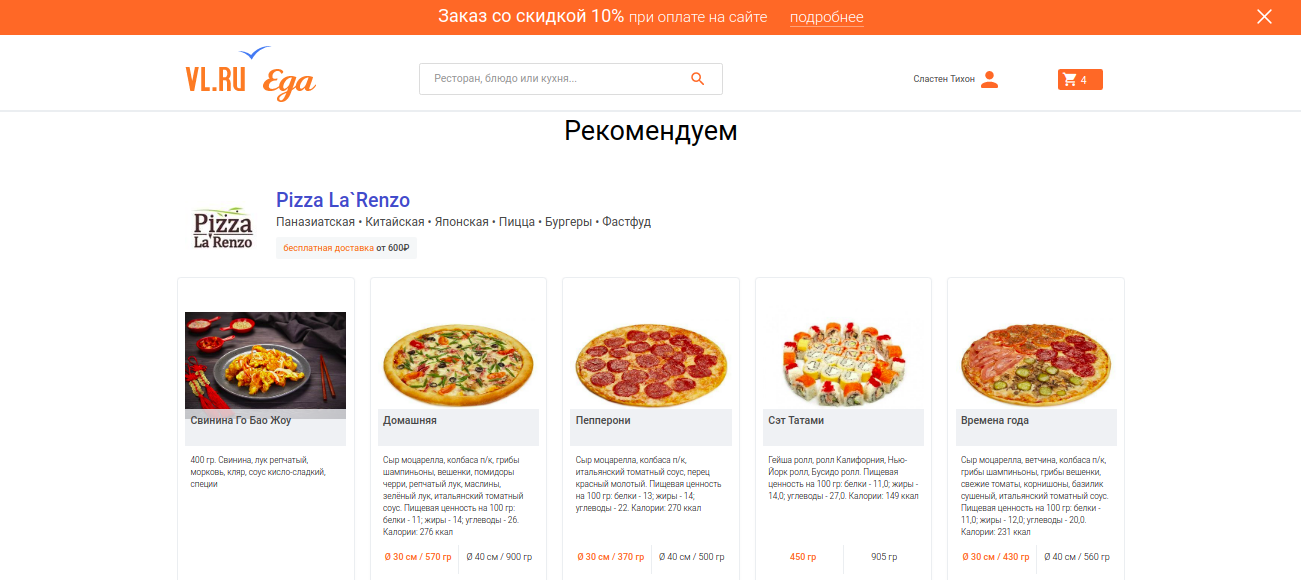
\includegraphics[scale=0.23]{images/tag_page.png}
    \caption{Процесс развертывания}
  \end{figure}
\end{frame}

\begin{frame}
  \frametitle{Заключение}
  \begin{itemize}
    \item Проведено сравнение моделей рекомендательных систем
    \item Рализован микро-сервис рекомендаций
    \item Рекомендации интегрированы на сайт "VLru Еда"
  \end{itemize}
\end{frame}

\end{document}
